\documentclass[11pt,a4paper]{article}

% Packages retained from the author's systematic-review format
\usepackage[utf8]{inputenc}
\usepackage[T1]{fontenc}
\usepackage{newtxtext,newtxmath}
\usepackage{geometry}
\geometry{left=1.5cm,right=1.5cm,top=2cm,bottom=2cm}
\usepackage{graphicx}
\usepackage{booktabs}
\usepackage{longtable}
\usepackage{array}
\usepackage{cite}
\usepackage{amsmath}
\usepackage{float}
\usepackage{enumitem}
\usepackage{xcolor}
\usepackage{multicol}
\usepackage{setspace}
\usepackage{tikz}
\usetikzlibrary{shapes.geometric,arrows.meta,positioning,backgrounds,fit}
\usepackage{hyperref}
\usepackage{microtype}

\hyphenpenalty=5000
\exhyphenpenalty=5000
\setlength{\emergencystretch}{2em}
\newcolumntype{L}[1]{>{\raggedright\arraybackslash}p{#1}}
\newcolumntype{C}[1]{>{\centering\arraybackslash}p{#1}}
\graphicspath{{../experiments/leakage_safe_validation/results/figures/}%
                 {../experiments/confirmatory_weekly_analysis/results/figures/}%
                 {../experiments/validation_integrity_audit/results/protocol_ladder/}%
                 {../experiments/validation_integrity_audit/results/external_wu_2026/}%
                 {../experiments/validation_integrity_audit/results/synthetic_stress_tests/}}

% Compact article layout
\setstretch{0.9}
\setlength{\parindent}{0.2cm}
\setlength{\parskip}{0pt}
\setlength{\columnsep}{0.55cm}
\hypersetup{
    colorlinks=true,
    linkcolor=blue,
    filecolor=magenta,
    urlcolor=blue,
    citecolor=blue
}
\setlist{
    nosep,
    leftmargin=*,
    itemsep=1pt,
    topsep=2pt,
    parsep=0pt,
    partopsep=0pt,
    label=--
}

\begin{document}

\begin{center}
{\large\textbf{Validation Integrity in Longitudinal Sports-Injury AI: An Executable Audit of Participant, Temporal, Selection, Calibration, and Observation Bias}}\\[0.7cm]

{\normalsize Marouane Aboutara-Belghiti$^{1}$, Mohamed Zeriab Es-sadek$^{1}$, Samir Belfkih$^{1}$}\\[0.3cm]

{\small $^{1}$ENSAM, Mohammed V University in Rabat, Morocco}\\
{\small Corresponding author: marouane\_aboutarabelghiti@um5.ac.ma}\\[0.3cm]
\end{center}

\begin{abstract}
\normalsize
Repeated observations, transductive preprocessing, supervised selection, and data-collection processes can inflate sports-injury AI performance. We developed a validation-integrity audit and tested it under controlled null conditions and in two runner cohorts. Simulations isolated participant memorization and global-selection leakage. Cohort 1 comprised 42,798 rows from 74 runners; its endpoint was retrospective classification of supplied injury-labelled event days, not forecasting. We evaluated a seven-rung protocol ladder, nested athlete-group validation, and all 21 non-overlapping temporal offsets. In cohort 2 (6,181 weekly samples; 142 runners), we crossed row-wise versus participant-grouped validation with global versus fold-local selection in 39- and 257-predictor matrices. Under null conditions, row-wise versus grouped ROC-AUC was 0.799 versus 0.491; global versus fold-local null-feature selection yielded 0.631 versus 0.502. In cohort 1, removing test-cohort statistics reduced ROC-AUC from 0.681 to 0.597 (paired change $-0.084$, 95\% CI $-0.177$ to $-0.008$). Natural-prevalence calibration reduced Brier score from 0.246 to 0.0157. Temporally de-overlapped ROC-AUC was 0.474-0.489. In cohort 2, random-forest row-wise versus grouped ROC-AUC was 0.730 versus 0.523 for 39 predictors (difference 0.207, 0.148-0.270) and 0.718 versus 0.586 for 257 predictors (0.132, 0.088-0.173). With grouping fixed, global selection inflated ROC-AUC by 0.052-0.065 across models. Validation design reversed conclusions under known ground truth and across cohorts and model families. Neither analysis establishes prospective warning utility. Validation integrity should be tested, not treated as a reporting detail.
\end{abstract}

\noindent\textbf{Keywords:} trustworthy artificial intelligence; sports injury; validation integrity; data leakage; grouped validation; feature selection; temporal overlap; calibration; reproducibility

\begin{multicols}{2}

%===========================================================================
\section{Introduction}
%===========================================================================

Sports-injury prediction is an appealing application of artificial intelligence (AI): an individualized warning could, in principle, support training-load modification, clinical review, or targeted recovery. Yet injury is rare, multifactorial, and embedded in longitudinal monitoring systems where observations from the same athlete are correlated. A large row count can therefore conceal a small effective sample, while inappropriate preprocessing or random row splitting can yield overoptimistic estimates. Recent evidence syntheses continue to identify limited external validation, heterogeneous outcome definitions, and incomplete reporting as central obstacles to reliable injury prediction in sport \cite{vaneetvelde2021,leckey2025}.

The public competitive-runners dataset introduced by L\"ovdal and colleagues is an important benchmark because it combines seven years of objective and subjective training logs from 74 runners and provides both daily and weekly representations \cite{lovdal2021,lovdaldataverse2021}. The original bagged-XGBoost system reported ROC-AUC 0.724 for a seven-day daily representation and 0.678 for a three-week aggregated representation \cite{lovdal2021}. However, a headline ROC-AUC does not establish that probabilities are reliable, alerts are useful, or the system will generalize to unseen athletes. These distinctions are particularly important at an injury-label prevalence near 1.3\%, where precision-recall analysis is more informative about positive predictions than ROC-AUC alone \cite{saito2015}.

Data leakage can arise throughout data collection, preprocessing, model fitting, calibration, and evaluation \cite{kapoor2023}. In longitudinal sports data, an additional problem is temporal pseudo-replication: adjacent target rows can share most of the same predictor history. A model may then exploit repeated or structurally sampled contexts without learning a temporally robust relationship. Reporting guidance for prediction models and risk-of-bias assessment consequently emphasizes explicit outcome definitions, predictor availability, clean validation separation, calibration, uncertainty, and open-science practices \cite{collins2024,moons2025}.

A recent athlete-independent analysis of the daily file from the same public dataset found weak discrimination and collapse toward chance after removing overlapping seven-day histories \cite{qiao2026}. The weekly data nevertheless require a separate audit because they reproduce the originally reported weekly result, aggregate 22 variables over three successive weeks, and exhibit a distinctive 21-day sampling structure. The present study therefore addresses five questions: (1) can the published weekly discrimination be reproduced; (2) which sequential validation safeguards change that conclusion; (3) does discrimination persist when adjacent three-week histories no longer overlap; (4) do calibrated predictions provide useful probability estimates or acceptable alert precision; and (5) do participant mixing and global supervised selection produce similar optimism in an independently collected runner cohort?

Our contribution is not another high-performing warning algorithm. The individual threats examined here---including participant mixing, test-transductive preprocessing, outcome-informed feature selection, prevalence-mismatched calibration, and temporal history overlap---are established methodological concerns. The contribution of this study is to operationalize these concerns as a reusable, claim-oriented validation-integrity audit for longitudinal prediction. The audit specifies seven domains, provides an executable stress test for each domain, and quantifies paired changes against a safeguarded reference pipeline. We evaluate the audit under controlled null conditions, reproduce a published weekly benchmark before correction, and examine whether the same validation sensitivities recur in an independently collected runner cohort. This design treats validation integrity as an empirical object of study rather than a reporting detail. Cohort 1 is analysed strictly as retrospective event-day classification.

%===========================================================================
\section{Methods}
%===========================================================================

We conducted a two-cohort methodological audit of open data and official replication materials. The analysis was designed around the principles of TRIPOD+AI and PROBAST+AI \cite{collins2024,moons2025}. Before model fitting, we defined the predictor-availability contract, independent resampling unit, primary metrics, and negative-control analyses. The second cohort tests whether the audit exposes the same class of validation sensitivity in independently collected data; because its predictors and endpoint construction differ, it is an external validation of the audit framework rather than transport validation of one fixed prediction model.

The official DataverseNL release contains training logs from a Dutch high-level middle- and long-distance running team observed from 2012 to 2019 \cite{lovdaldataverse2021}. The weekly file used here contains 42,798 athlete-date rows from 74 athletes, including 575 rows labelled as injury (prevalence 1.3435\%). Its MD5 checksum, \texttt{5fe8c80e2a2fa267789be363aacad43a}, matched the value published by the repository.

Each target row contains aggregate training-load and subjective-response summaries for three preceding weekly windows. The source outcome does not include anatomical site, diagnosis, onset mechanism, severity, recovery, or incident-episode identifier. We therefore use the term \emph{injury-labelled event day} and evaluate retrospective event-day classification. A provisional 28-day future target developed during exploratory work was excluded from the confirmatory analysis because the released event-centred table did not demonstrate continuous prospective follow-up.

The independent cohort was the processed supplementary release of Wu and colleagues \cite{wu2026}. It contains 6,181 weekly samples from 142 UK endurance runners prospectively monitored for 12 months, including 564 positive labels. We evaluated both official matrices: 39 evidence-prioritized predictors and all 257 available predictors. The workbooks contain neither an explicit participant identifier nor a week field. Five invariant baseline fields sex, age, prior lower-limb injury days, average running hours, and interval-training frequency , jointly identified exactly 142 unique and 142 contiguous row trajectories in both matrices. We therefore used this explicitly labelled \emph{inferred participant identifier} for grouped validation. This permits an identity-separation audit but not chronological validation.

The sampling audit reconstructed runs of positive labels and inspected spacing between retained records. There were 389 injury-label run starts; 347 (89.2\%) occurred exactly 22 date units after the preceding retained row, and all 389 had zero retained rows in the implied preceding 21-day history. Moreover, the provisional future-label experiment generated 2,245 positive rows 22-28 date units before a future retained injury label, while 7,241 provisional negatives lacked a complete retained-observation sequence over the next 28 units. These patterns prevented a defensible prospective risk-set definition.

The primary feature contract retained 66 numeric predictors. Athlete identifier, date, outcome, recording-gap variables, and three supplied relative-load ratios were excluded. The ratios were reserved for sensitivity analysis because extreme values can be driven by small denominators. Recording gap was introduced only as a prohibited-feature leakage stress test, never as a candidate predictor. True negative controls were generated by within-athlete label permutation and circular shifting.

Figure~\ref{fig:workflow} summarizes the analysis. The primary validation kept every athlete entirely within one fold. All preprocessing, hyperparameter selection, probability calibration, and threshold selection occurred without access to outer-test outcomes. Complete out-of-fold predictions were retained so every headline result could be traced to an untouched prediction.

\end{multicols}

\begin{figure}[H]
\centering
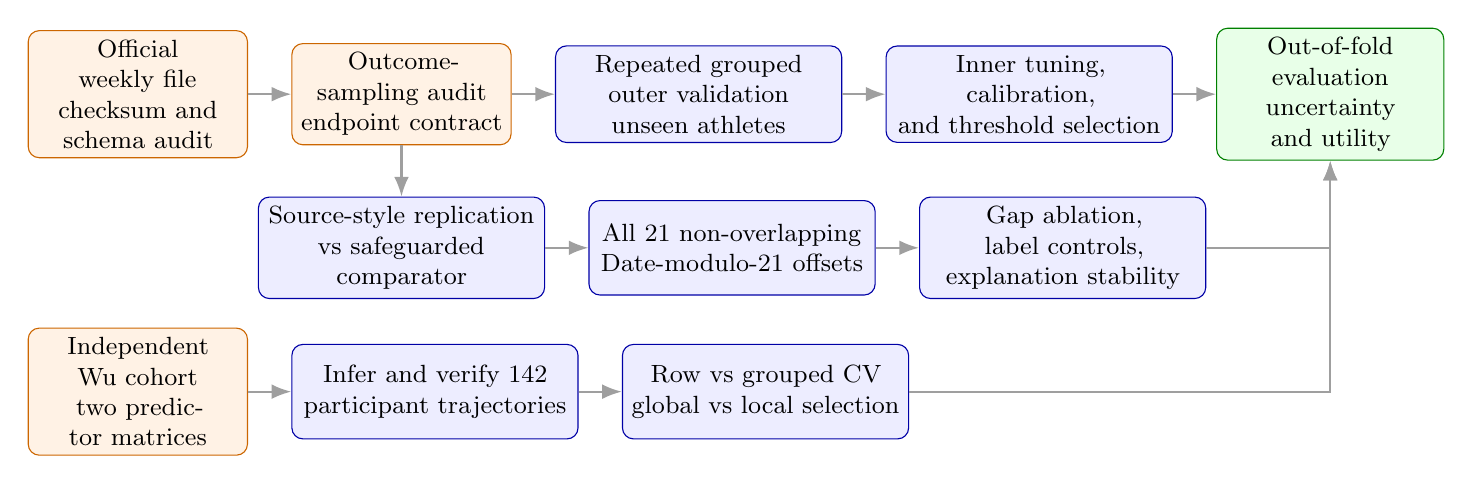
\begin{tikzpicture}[
    node distance=0.55cm and 0.55cm,
    box/.style={rectangle,rounded corners,draw=blue!65!black,fill=blue!7,
                minimum height=1.2cm,text width=3.4cm,align=center,font=\small},
    audit/.style={rectangle,rounded corners,draw=orange!80!black,fill=orange!10,
                  minimum height=1.05cm,text width=2.55cm,align=center,font=\small},
    result/.style={rectangle,rounded corners,draw=green!50!black,fill=green!9,
                   minimum height=1.05cm,text width=2.65cm,align=center,font=\small},
    arrow/.style={-{Latex[length=2.5mm]},thick,draw=gray!75}
]
\node[audit] (data) {Official weekly file\\checksum and schema audit};
\node[audit,right=of data] (outcome) {Outcome-sampling audit\\endpoint contract};
\node[box,right=of outcome] (outer) {Repeated grouped outer validation\\unseen athletes};
\node[box,right=of outer] (inner) {Inner tuning, calibration,\\and threshold selection};
\node[result,right=of inner] (eval) {Out-of-fold evaluation\\uncertainty and utility};

\node[box,below=0.65cm of outcome] (rep) {Source-style replication\\vs safeguarded comparator};
\node[box,right=of rep] (nonoverlap) {All 21 non-overlapping\\Date-modulo-21 offsets};
\node[box,right=of nonoverlap] (controls) {Gap ablation, label controls,\\explanation stability};

\node[audit,below=2.15cm of data] (external) {Independent Wu cohort\\two predictor matrices};
\node[box,right=of external] (identity) {Infer and verify 142\\participant trajectories};
\node[box,right=of identity] (extaudit) {Row vs grouped CV\\global vs local selection};

\draw[arrow] (data) -- (outcome);
\draw[arrow] (outcome) -- (outer);
\draw[arrow] (outer) -- (inner);
\draw[arrow] (inner) -- (eval);
\draw[arrow] (outcome) -- (rep);
\draw[arrow] (rep) -- (nonoverlap);
\draw[arrow] (nonoverlap) -- (controls);
\draw[arrow] (controls.east) -| (eval.south);
\draw[arrow] (external) -- (identity);
\draw[arrow] (identity) -- (extaudit);
\draw[arrow] (extaudit.east) -| (eval.south);
\end{tikzpicture}
\caption{Two-cohort validation-integrity architecture}
\label{fig:workflow}
\end{figure}

\subsection{Reusable validation-integrity profile}
\label{sec:vip}

We formalized the audit as the seven-domain validation-integrity profile
(Table~\ref{tab:vip}). The profile is a protocol, not a numerical score. Each domain is
reported as \emph{verified}, \emph{violated}, \emph{indeterminate}, or
\emph{not applicable}, together with executable evidence. This prevents a
high aggregate score from concealing one claim-invalidating failure.

\begin{table}[H]
\centering
\scriptsize
\caption{Reusable Validation-Integrity Profile for longitudinal prediction AI.}
\label{tab:vip}
\begin{tabular}{L{1.1cm} L{2.8cm} L{4.1cm} L{4.0cm} L{3.2cm}}
\toprule
\textbf{Code} & \textbf{Domain} & \textbf{Validity condition} & \textbf{Executable audit} & \textbf{Required evidence} \\
\midrule
E & Endpoint and index time & The target, prediction time, risk set, and predictor availability are unambiguous. & Reconstruct episodes and observation spacing; reject future targets without continuous follow-up. & Endpoint contract; exclusions; sampling diagram. \\
I & Identity separation & Every correlated identity unit belongs to only one side of an evaluation split. & Count participant overlap in every fold; compare row-wise with grouped out-of-fold estimates. & Group definition; split manifest; paired metric change. \\
T & Transformation locality & Imputation, scaling, normalization, and representation statistics use training data only. & Replace label-conditioned and test-transductive transformations sequentially. & Fitted-statistic provenance; protocol ladder. \\
S & Supervised-selection locality & Every outcome-informed selection or tuning operation is repeated inside training folds. & Compare global with fold-local selection under an otherwise fixed grouped design. & Selected features by fold; paired metric change. \\
C & Calibration integrity & Calibration units are independent of fitting/test units and reflect the target prevalence. & Measure fit--calibration identity/row overlap; compare balanced with natural-prevalence calibration. & Calibration split; prevalence; Brier, log loss, intercept, slope. \\
H & History independence & Test histories do not duplicate or substantially overlap training/evaluation histories beyond the deployment scenario. & Evaluate all prespecified non-overlapping temporal offsets or forward-chaining splits. & Window map; offset results; no performance-selected offset. \\
O & Observation-process resistance & Administrative availability or post-event proxies cannot determine the label. & Prohibited-feature stress test plus refitted within-identity permutation and circular-shift controls. & Feature-availability contract; null distributions. \\
\bottomrule
\end{tabular}
\end{table}

Application follows five steps: define the intended claim and endpoint contract;
map identities, time windows, and all outcome-informed operations; construct the
safeguarded reference pipeline; vary one integrity domain at a time while
holding the model family and evaluation rows fixed where possible; and report
paired cluster-aware changes for discrimination and probability accuracy. For
metric $m$ and stress condition $d$, the audit quantity is
\begin{equation}
\Delta_{m,d}=m(\widehat{p}_{d})-m(\widehat{p}_{\mathrm{reference}}),
\end{equation}
where both predictions are aligned to the same evaluation rows and uncertainty
is resampled at the independent identity unit. The sign is interpreted in the
metric's direction; the profile does not assume that effects are additive or causal.


\begin{multicols}{2}

We first constructed a version-compatible replication of the official weekly notebook. The last 10 athlete identifiers formed the test set. For fidelity, each athlete was normalized using that athlete's healthy rows, nine XGBoost models were fitted to balanced samples drawn with replacement, Platt calibration used another balanced sample from the same development-row pool, and a threshold sample was drawn from that pool. This comparator intentionally preserves two problematic properties of the source workflow: test outcomes identify healthy test rows for normalization, and the row pools used for model fitting and calibration can overlap. It is reported solely to reproduce the original result.

The safeguarded comparator used the same final 10 test athletes but restricted preprocessing to training information, removed the three ratio variables, separated model-fitting and calibration athletes, and left test athletes untouched. Both workflows were repeated five times, each with nine XGBoost bags and 2,048 sampled rows per class where available. For the paired comparison, probabilities were averaged across the five stochastic runs for each test row.

To locate where the conclusion changed, we evaluated seven prespecified protocol rungs on the same final 10 test athletes. Starting from the source-style workflow, we sequentially introduced: (S1) outcome-blind but still transductive within-athlete normalization using all test rows; (S2) no test-cohort distribution statistics; (S3) athlete-disjoint fitting and calibration pools; (S4) the safe feature contract; (S5) calibration at the natural development prevalence; and (S6) fitting on all naturally occurring rows with class weighting instead of balanced row resampling. Every rung retained five stochastic experiments and nine XGBoost bags. Paired 95\% intervals used 5,000 athlete-cluster bootstrap samples after averaging repeated predictions per row. Because design choices interact, adjacent changes are protocol-step contrasts and are not interpreted as causal component effects.

We used two null simulations to verify that the audit detects known failure mechanisms. The identity-only scenario generated 100 participants with 30 repeated rows each. Injury propensity varied randomly between participants, while eight invariant participant fingerprints and eight dynamic noise variables were independent of that propensity; no signal could generalize to a new participant. Random-forest performance under random row and participant-grouped five-fold validation was compared. The selection-only scenario generated 3,000 independent rows, a 10\% random outcome, and 300 null predictors. Logistic regression used the 20 predictors with the largest univariate $F$ statistics selected either once from the complete dataset or separately within every training fold. Each scenario was regenerated 50 times. The population-generalizable ROC-AUC was 0.5 by construction.

In the Wu cohort, we crossed identity separation with supervised feature-selection locality. Five protocols were evaluated: stratified random row cross-validation with global selection, row cross-validation with fold-local selection, participant-grouped validation with global selection, grouped validation with fold-local selection, and grouped validation using all available features. Global selection used the outcome from the complete matrix and was included only as a deliberately biased stress condition. Fold-local selection used a univariate training-fold $F$ statistic to retain 20 predictors; the number was fixed before evaluation. Logistic regression, random forest, and XGBoost used locked hyperparameters so that validation design, rather than differential tuning budgets, was the experimental factor. Each condition used five folds repeated three times. Predictions were averaged by released row across repetitions, and 95\% intervals used 2,000 inferred-participant cluster bootstrap samples. We report ROC-AUC, AP, Brier score, log loss, calibration intercept and slope, and expected calibration error. Reconstruction robustness was tested using exact four- and five-field fingerprints, contiguous three-field runs, and a conservative exact three-field rule that merged trajectories.

The primary analysis compared L2-regularized logistic regression, random forest, and XGBoost. We used five outer athlete-group folds repeated three times. Within each outer-training partition, three-fold grouped validation selected hyperparameters, preventing model-selection information from entering the outer performance estimate \cite{cawley2010}. Base-model inner out-of-fold probabilities were then used to select no calibration, Platt scaling, or isotonic regression by Brier score. A classification threshold was selected from cross-calibrated inner predictions by maximizing the Matthews correlation coefficient (MCC). The selected pipeline was refitted without using the outer-test outcomes.

Adjacent rows may share nearly all of their 21-day predictor histories. We therefore evaluated every subset defined by $\mathrm{Date}\bmod 21=k$, for $k=0,\ldots,20$. Within each offset, all three models were refitted under three repeated athlete-group allocations, yielding 63 conditions per model and 189 conditions overall. Model settings were locked from the preceding nested analysis; no offset was selected according to performance. Two-sided Wilcoxon signed-rank tests compared offset-averaged ROC-AUC with 0.5 and average precision with offset-specific prevalence.

The observation-process ablation evaluated the safe feature set, recording gap alone, and safe features plus recording gap under identical grouped splits. Label controls used 100 full grouped-logistic refits for each of two null mechanisms: random permutation of labels within athlete and circular shifting of each athlete's label sequence. Empirical one-sided probabilities were calculated as $(1+b)/(1+100)$, where $b$ is the number of null values at least as large as the observed value. The three supplied ratios were reintroduced only in a prespecified sensitivity analysis.

Primary metrics were ROC-AUC, average precision (AP), Brier score, and MCC. We additionally reported calibration intercept and slope, precision, recall, specificity, and alert rate. Brier skill was computed relative to a fold-training prevalence forecast:
\begin{equation}
\mathrm{BSS}=1-\frac{\mathrm{Brier}_{\mathrm{model}}}
{\mathrm{Brier}_{\mathrm{prevalence}}}.
\end{equation}
Because the outcome was rare, AP and precision were interpreted relative to the 1.3435\% prevalence baseline \cite{saito2015}. Calibration was evaluated separately from discrimination because a ranking model can still produce unreliable risk estimates \cite{vancalster2019}.

Repeated outer predictions for each original row were averaged before pooled evaluation. Ninety-five per cent confidence intervals used 2,000 athlete-cluster bootstrap samples. The source-style versus safeguarded comparison used 5,000 paired athlete-bootstrap samples from the 10 shared test athletes. Fixed budgets of 1, 2, 5, and 10 alerts per 100 rows were evaluated with 1,000 athlete-bootstrap samples. Feature rankings were calculated independently for each of 15 repeated outer fits and summarized using pairwise Spearman correlation and top-10 Jaccard overlap. Rankings were treated as model-reliance summaries, not causal risk factors.

Analyses were implemented in Python using NumPy, SciPy, scikit-learn, Matplotlib, pandas, and XGBoost \cite{harris2020,virtanen2020,pedregosa2011,hunter2007,chen2016}. Prespecified master seeds of 20260829 and 20260830 were used for the original and independent-cohort analyses. The reproducibility package contains exact dependency versions, source-data hashes, feature manifests, split assignments, inner-selection results, all out-of-fold probabilities, bootstrap summaries, protocol contrasts, robustness outputs, and figure-generation code.

%===========================================================================
\section{Results}
%===========================================================================

Table~\ref{tab:primary} presents pooled repeated nested-validation results. Discrimination was modest for all three models: ROC-AUC ranged from 0.592 to 0.615 and AP from 0.0172 to 0.0182. Although the AP estimates exceeded prevalence numerically, their absolute improvement was small. Random forest exceeded XGBoost in paired ROC-AUC by 0.0236 (95\% CI 0.0010-0.0432) and MCC by 0.0101 (0.0013-0.0178), but not in AP or Brier score. There was no clear paired difference between logistic regression and random forest.

\end{multicols}

\begin{table}[H]
\centering
\small

\begin{tabular}{L{3.0cm} C{2.4cm} C{2.4cm} C{2.4cm} C{2.4cm} C{2.4cm}}
\toprule
\textbf{Model} & \textbf{ROC-AUC} & \textbf{Average precision} & \textbf{Brier score} & \textbf{MCC} & \textbf{Alerts/100} \\
\midrule
Logistic regression & 0.608 (0.580-0.639) & 0.0177 (0.0148-0.0220) & 0.01327 (0.01103-0.01597) & 0.0418 (0.0270-0.0581) & 43.1 (36.7-48.9) \\
Random forest & 0.615 (0.581-0.654) & 0.0182 (0.0147-0.0235) & 0.01323 (0.01083-0.01589) & 0.0455 (0.0294-0.0620) & 49.2 (42.7-55.3) \\
XGBoost & 0.592 (0.558-0.625) & 0.0172 (0.0138-0.0234) & 0.01324 (0.01083-0.01593) & 0.0354 (0.0195-0.0523) & 41.4 (35.2-47.7) \\
\bottomrule
\end{tabular}
\caption{Leakage-safe repeated nested-validation performance}
\label{tab:primary}
\end{table}

\begin{multicols}{2}

At the inner-selected MCC thresholds, precision was 1.90\%, 1.88\%, and 1.83\% for logistic regression, random forest, and XGBoost. Thus, approximately 98 of every 100 alerts were false positives. Calibration slopes were 0.816 (95\% CI 0.576-1.265), 0.965 (0.690-1.310), and 0.972 (0.615-1.379), respectively. The intervals were wide, reflecting the limited number of independent athletes. Full-window Brier skill was $-0.0007$, 0.0020, and 0.0015, indicating almost no probability-accuracy improvement over the fold-training prevalence forecast.

Across five source-style replications, mean ROC-AUC was 0.677 (SD 0.002), closely reproducing the published weekly ROC-AUC of 0.678. Mean AP was 0.091 (SD 0.019), but mean Brier score was 0.160 (SD 0.0068). The safeguarded workflow produced mean ROC-AUC 0.540 (SD 0.082), AP 0.0222 (SD 0.0054), and Brier score 0.0157.

After averaging the five predictions per test row, source-style and safeguarded ROC-AUC were 0.679 and 0.577. The paired difference was 0.102 (95\% CI 0.027-0.199). The AP difference was 0.061 (0.008-0.117). In the opposite direction, the source-style Brier score was worse by 0.143 (0.127-0.160). Consequently, the source workflow increased apparent ranking performance while producing substantially less accurate probabilities.

\end{multicols}

\begin{figure}[H]
\centering
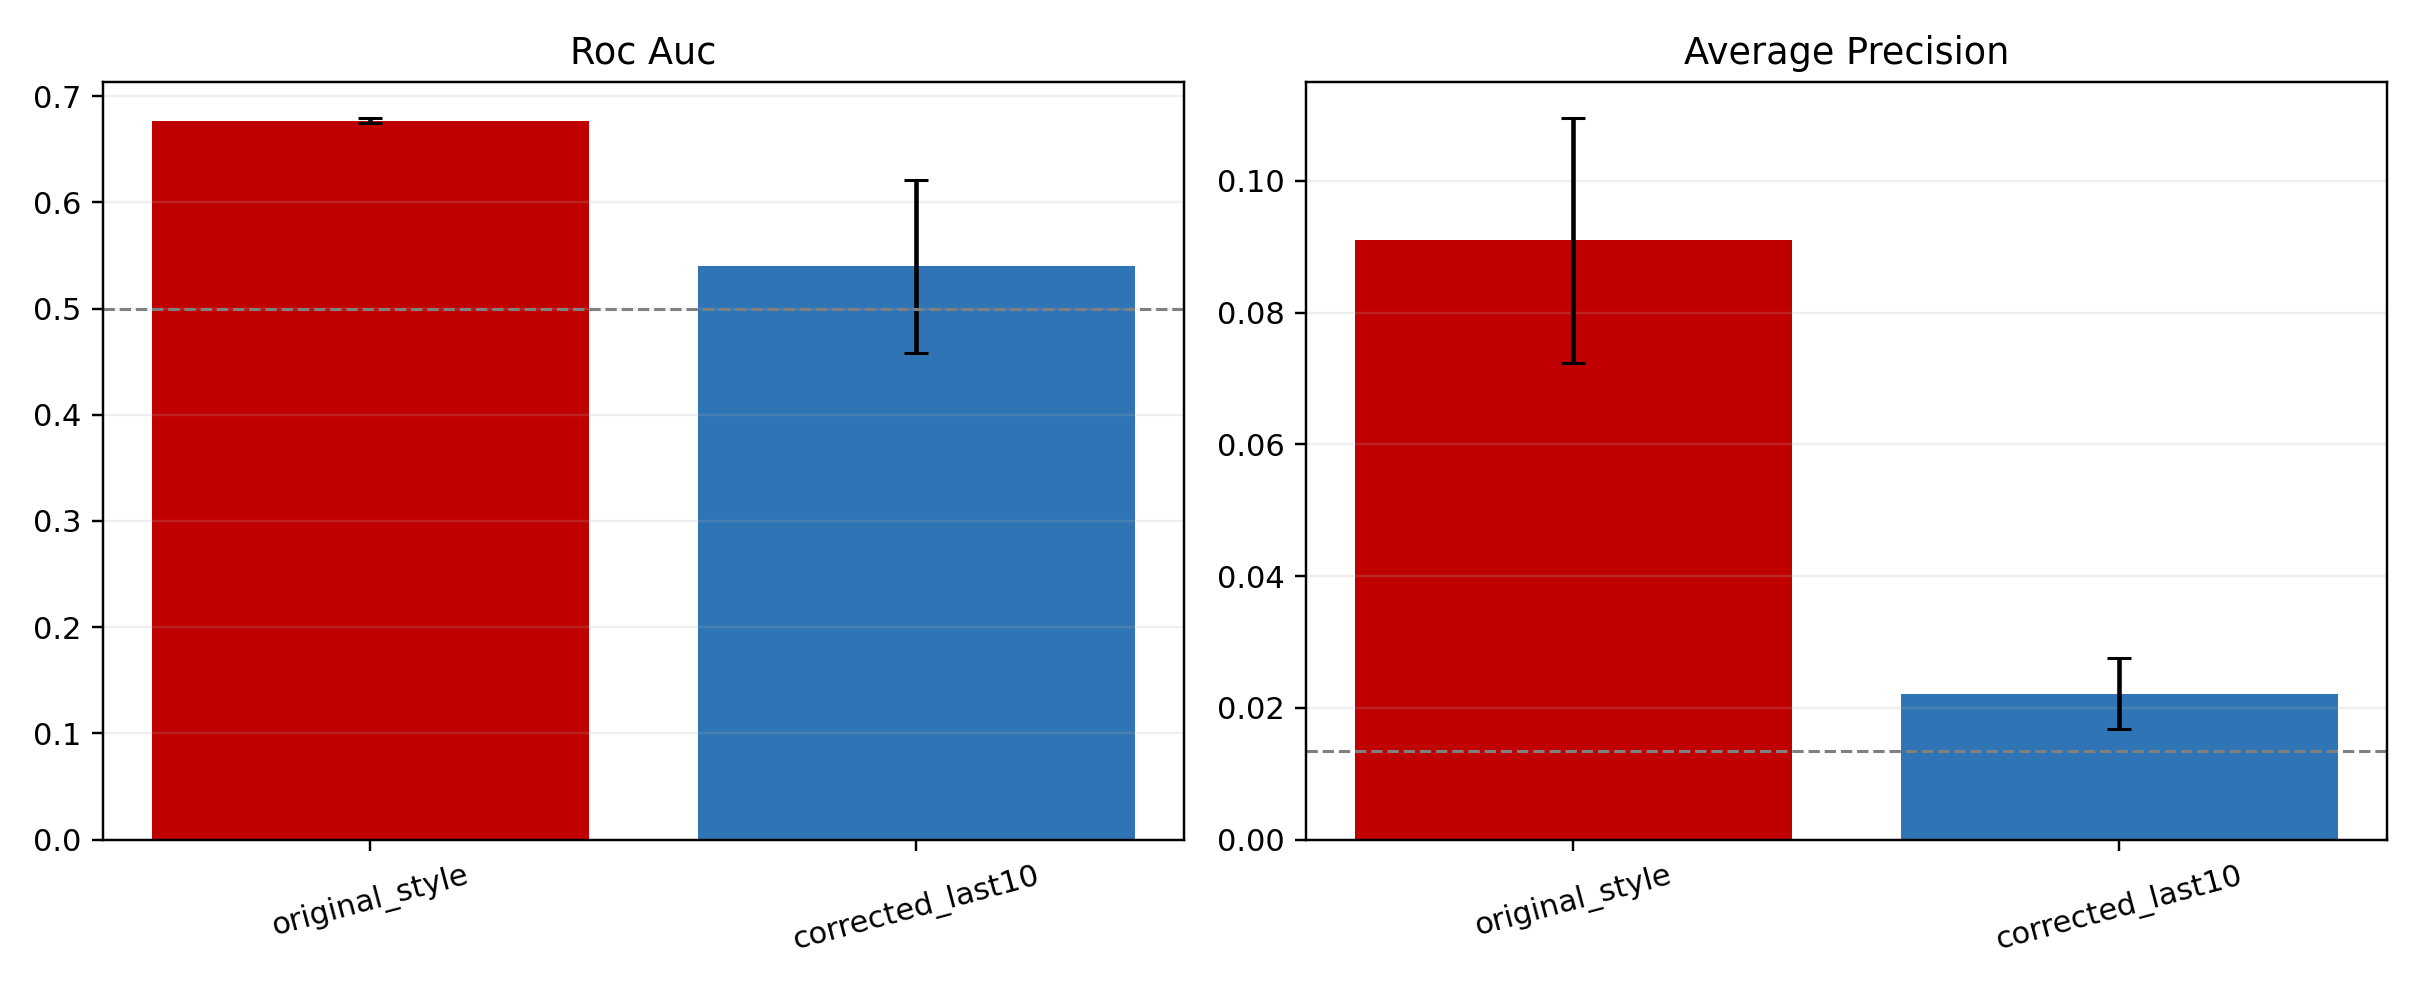
\includegraphics[width=0.77\textwidth]{original_vs_corrected.png}
\caption{Five source-style replications and five safeguarded replications on the same final 10 athletes}
\label{fig:originalcorrected}
\end{figure}

\begin{multicols}{2}

The protocol ladder isolated a decisive change in the evaluation conclusion (Figure~\ref{fig:ladder}). Replacing healthy-row normalization with outcome-blind within-athlete normalization did not reduce discrimination: ROC-AUC changed from 0.675 to 0.681 (paired change 0.007, 95\% CI $-0.001$-0.012). Removing all test-cohort distribution statistics reduced ROC-AUC to 0.597 (change $-0.084$, $-0.177$ to $-0.008$) and AP from 0.103 to 0.026 (change $-0.078$, $-0.171$ to $-0.013$). Thus, test-outcome conditioning itself was unacceptable, but access to the test athletes' feature distributions, even without their outcomes was the component most clearly associated with inflated ranking in this comparison.

Separating fitting and calibration athletes produced ROC-AUC 0.591; safe-feature restriction left it at 0.593. Balanced calibration yielded Brier scores near 0.246 on the natural-prevalence test set. Restoring natural-prevalence calibration reduced Brier score to 0.0157 (paired change $-0.2303$, $-0.2756$ to $-0.1851$) without improving discrimination. Fitting all natural rows with class weighting yielded ROC-AUC 0.620 (0.501-0.743), AP 0.0250 (0.0143-0.0668), and Brier score 0.0156 (0.0097-0.0213). The wide intervals reflect only 10 independent test athletes.

\end{multicols}

\begin{figure}[H]
\centering
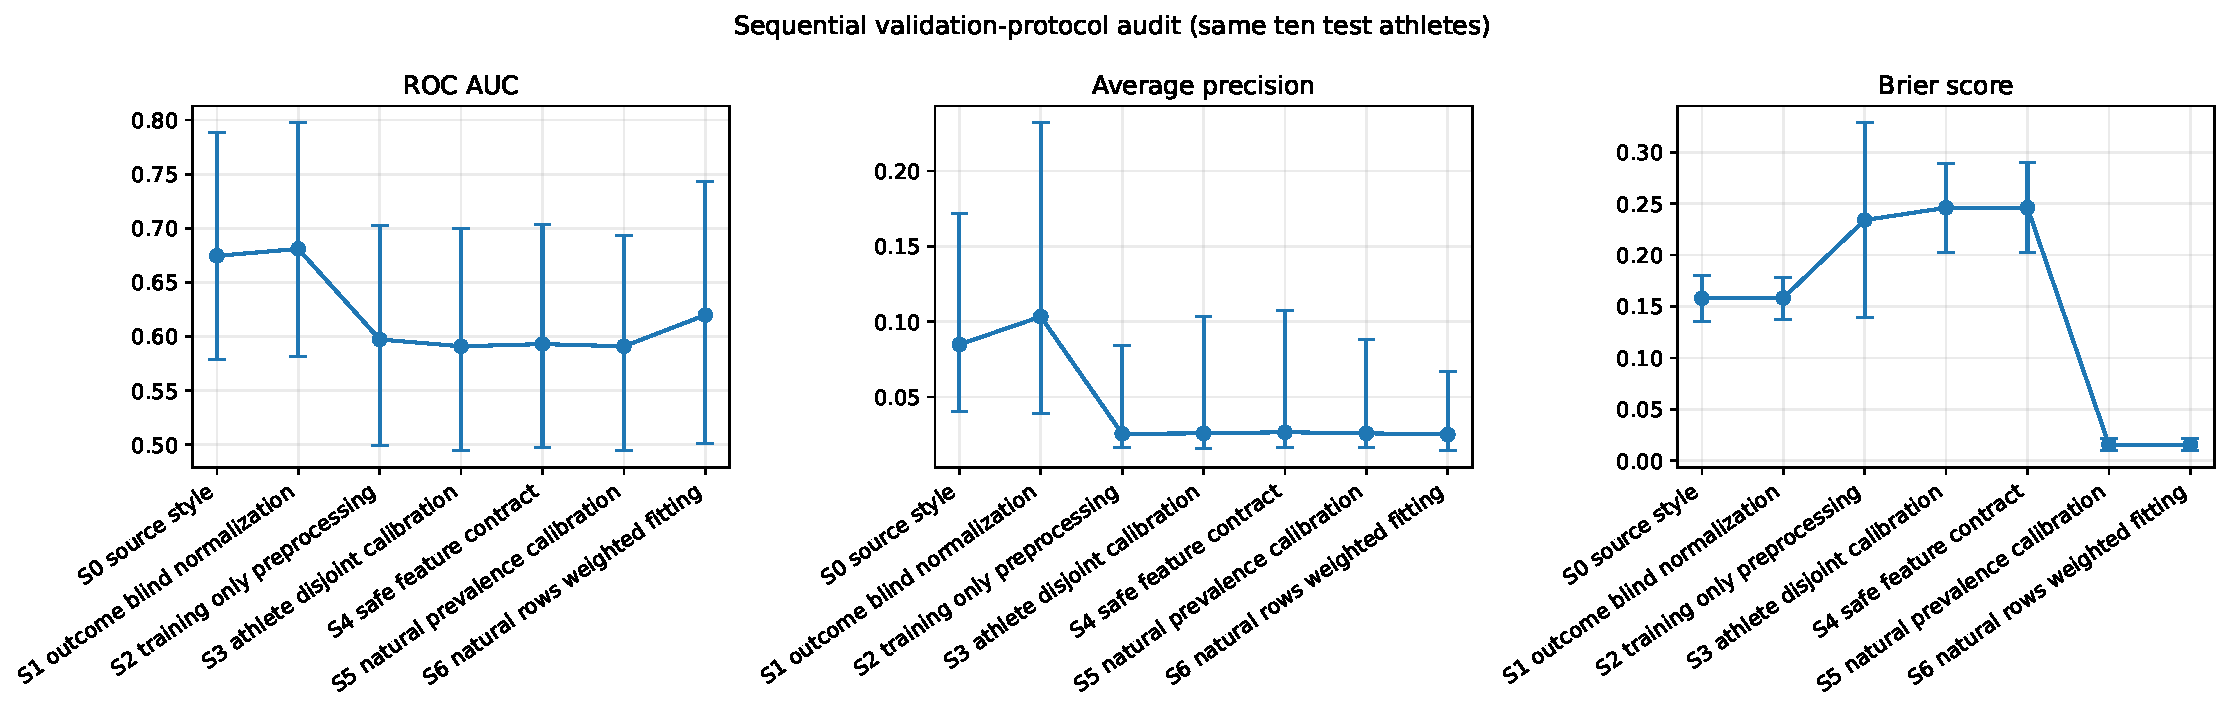
\includegraphics[width=0.94\textwidth]{protocol_ladder.pdf}
\caption{Sequential validation-protocol ladder on the same final 10 athletes}
\label{fig:ladder}
\end{figure}

\begin{multicols}{2}

The controlled simulations recovered both prespecified failure mechanisms (Figure~\ref{fig:synthetic}). In the identity-only scenario, random row validation produced mean ROC-AUC 0.799 (SD 0.029), despite fingerprints being independent of participant risk. Participant-grouped validation returned mean ROC-AUC 0.491 (SD 0.043), consistent with the true unseen-participant value of 0.5. Mean AP was 0.475 under row validation and 0.161 under grouping.

In the selection-only scenario, choosing 20 of 300 null predictors on the complete dataset before cross-validation yielded mean ROC-AUC 0.631 (SD 0.012) and AP 0.163. Repeating selection inside each training fold returned ROC-AUC 0.502 (SD 0.029) and AP 0.103, close to the 10\% prevalence. These controlled results demonstrate that the audit can detect optimism when population-generalizable signal is absent by construction.

\end{multicols}

\begin{figure}[H]
\centering
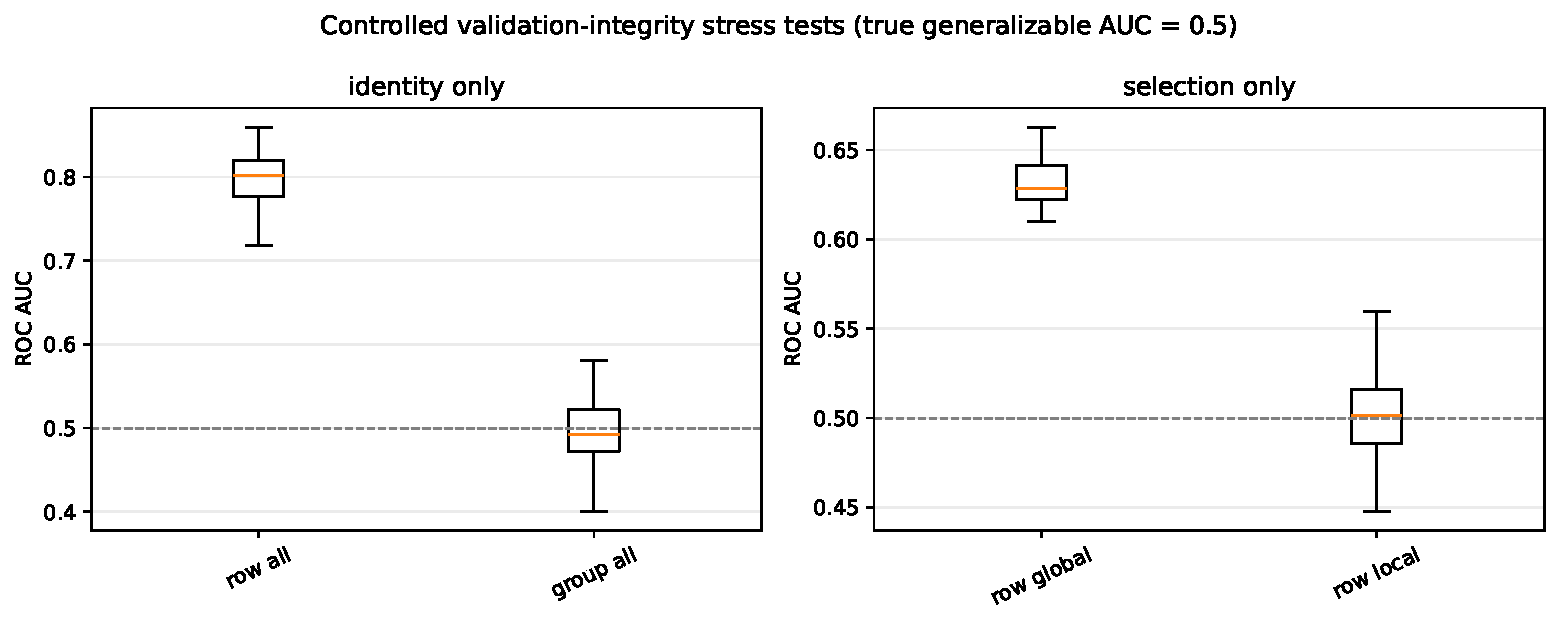
\includegraphics[width=0.78\textwidth]{synthetic_stress_tests.pdf}
\caption{Fifty controlled replications of identity and supervised-selection leakage}
\label{fig:synthetic}
\end{figure}

\begin{multicols}{2}

The independently collected Wu cohort reproduced the validation-design sensitivity (Table~\ref{tab:external}). In the 39-predictor matrix, random-forest ROC-AUC was 0.730 under random row validation with fold-local selection but 0.523 under participant-grouped fold-local validation, a paired difference of 0.207 (95\% participant-bootstrap CI 0.148-0.270). XGBoost fell from 0.706 to 0.558 (difference 0.148, 0.103-0.194), and logistic regression from 0.656 to 0.613 (difference 0.044, 0.023-0.066). Every random row fold shared 128-134 of 142 inferred participants between training and test data; every grouped fold had zero overlap.

The 257-predictor matrix showed the same model-agnostic pattern: row-wise versus grouped fold-local ROC-AUC differences were 0.053 (0.027-0.075), 0.132 (0.088-0.173), and 0.130 (0.090-0.173) for logistic regression, random forest, and XGBoost. Supervised selection locality also mattered. With participant grouping fixed, global rather than fold-local selection increased ROC-AUC by 0.052 (0.029-0.075), 0.053 (0.021-0.084), and 0.065 (0.030-0.102), respectively. Thus, participant grouping and fold-local selection addressed distinct optimism mechanisms.

The identity reconstruction was internally robust. Exact four- and five-field fingerprints and contiguous runs defined by the first three fields produced the identical 142-trajectory partition in both matrices. A conservative three-field exact rule merged these into 134 groups. Repeating grouped fold-local validation under this coarser rule did not improve the estimates: ROC-AUC ranged from 0.518 to 0.596 for the 39-predictor matrix and from 0.545 to 0.630 for the 257-predictor matrix. Full reconstruction proofs and 2,000-group-bootstrap intervals are provided in the supplement.

\end{multicols}

\begin{table}[H]
\centering
\scriptsize

\begin{tabular}{L{2.5cm} L{2.3cm} C{2.7cm} C{2.7cm} C{2.7cm} C{2.7cm}}
\toprule
\textbf{Matrix} & \textbf{Model} & \textbf{Row CV ROC-AUC} & \textbf{Grouped ROC-AUC} & \textbf{Row CV AP} & \textbf{Grouped AP} \\
\midrule
39 predictors & Logistic & 0.656 (0.599-0.702) & 0.613 (0.561-0.658) & 0.177 (0.129-0.234) & 0.151 (0.112-0.191) \\
39 predictors & Random forest & 0.730 (0.680-0.769) & 0.523 (0.472-0.574) & 0.241 (0.174-0.296) & 0.103 (0.081-0.131) \\
39 predictors & XGBoost & 0.706 (0.654-0.750) & 0.558 (0.509-0.602) & 0.221 (0.162-0.272) & 0.114 (0.089-0.145) \\
257 predictors & Logistic & 0.697 (0.653-0.734) & 0.644 (0.605-0.681) & 0.204 (0.141-0.261) & 0.143 (0.113-0.183) \\
257 predictors & Random forest & 0.718 (0.668-0.759) & 0.586 (0.542-0.632) & 0.232 (0.164-0.293) & 0.128 (0.098-0.173) \\
257 predictors & XGBoost & 0.704 (0.655-0.744) & 0.574 (0.524-0.618) & 0.228 (0.159-0.290) & 0.125 (0.093-0.166) \\
\bottomrule
\end{tabular}
\caption{Independent Wu-cohort audit using fold-local supervised feature selection. Values are pooled repeat-averaged estimates (95\% inferred-participant cluster-bootstrap CI). Random-row folds contain the same participants on both sides; grouped folds contain no participant overlap.}
\label{tab:external}
\end{table}

\begin{figure}[H]
\centering
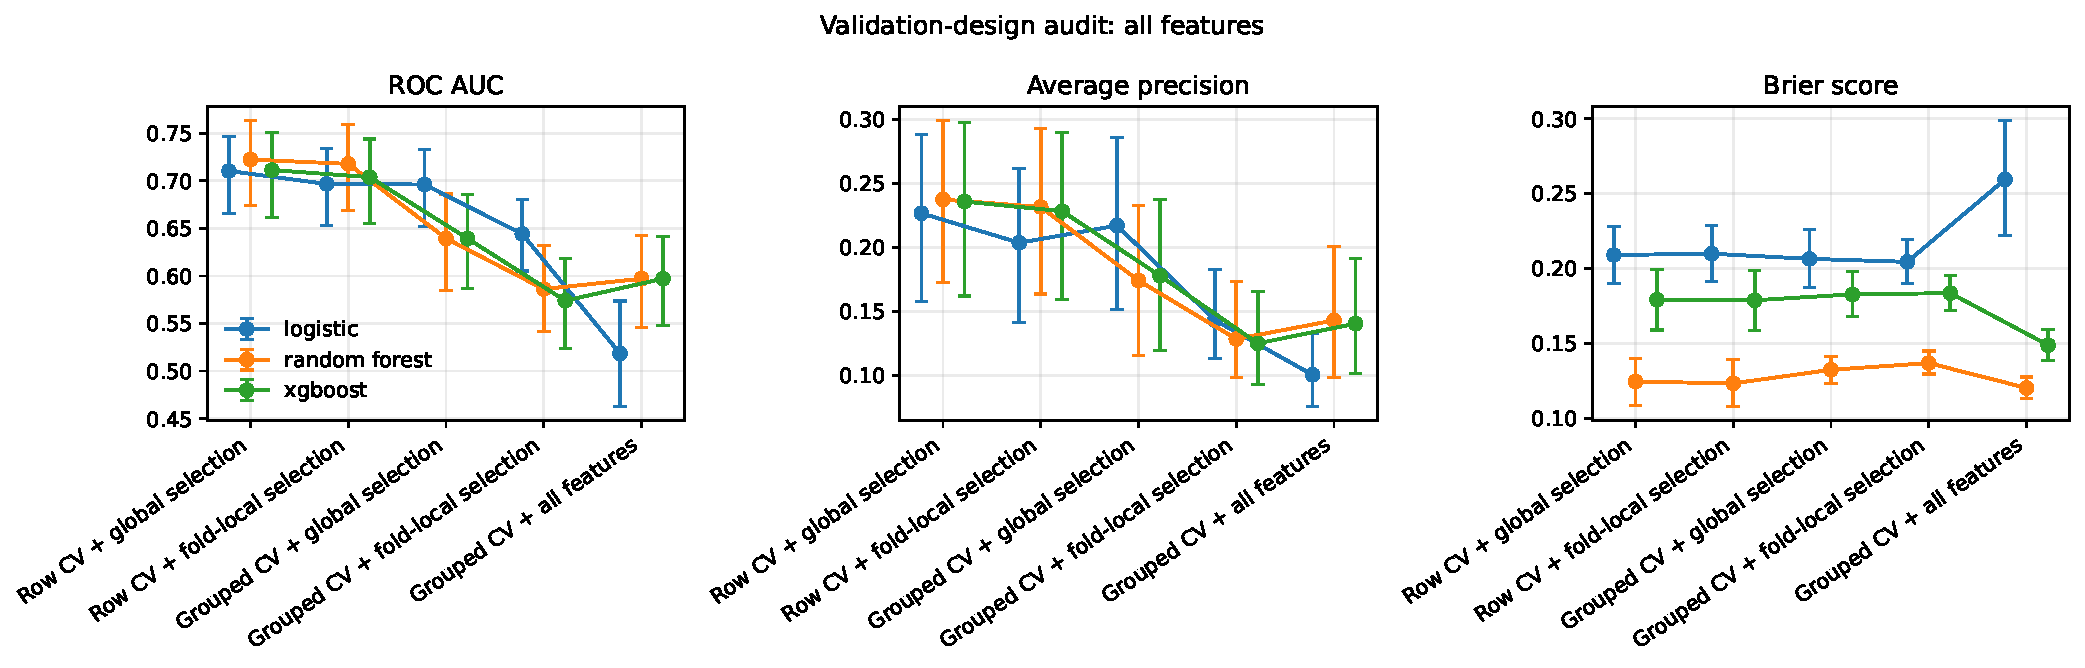
\includegraphics[width=0.96\textwidth]{validation_audit_all_features.pdf}
\caption{Independent-cohort validation audit for the 257-predictor matrix}
\label{fig:externalaudit}
\end{figure}

\begin{multicols}{2}


Removing adjacent overlap changed the interpretation of every model (Table~\ref{tab:nonoverlap}). Mean ROC-AUC across the 21 offsets fell by 0.122 for logistic regression, 0.127 for random forest, and 0.118 for XGBoost. None differed reliably from chance across offsets. AP did not reliably exceed offset-specific prevalence, and mean Brier skill remained approximately zero.

\end{multicols}

\begin{table}[H]
\centering
\small

\begin{tabular}{L{3.1cm} C{2.5cm} C{2.0cm} C{2.7cm} C{2.0cm} C{2.5cm}}
\toprule
\textbf{Model} & \textbf{ROC-AUC} & \textbf{$p$ vs 0.5} & \textbf{Average precision} & \textbf{$p$ vs prevalence} & \textbf{Mean Brier skill} \\
\midrule
Logistic regression & 0.485 (0.097) & 0.517 & 0.0158 (0.0076) & 0.191 & $-0.00067$ \\
Random forest & 0.489 (0.104) & 0.495 & 0.0185 (0.0129) & 0.103 & 0.00036 \\
XGBoost & 0.474 (0.100) & 0.096 & 0.0181 (0.0104) & 0.050 & $-0.00052$ \\
\bottomrule
\end{tabular}
\caption{Performance across all 21 non-overlapping weekly offsets and three athlete-group repetitions per offset}
\label{tab:nonoverlap}
\end{table}

\begin{figure}[H]
\centering
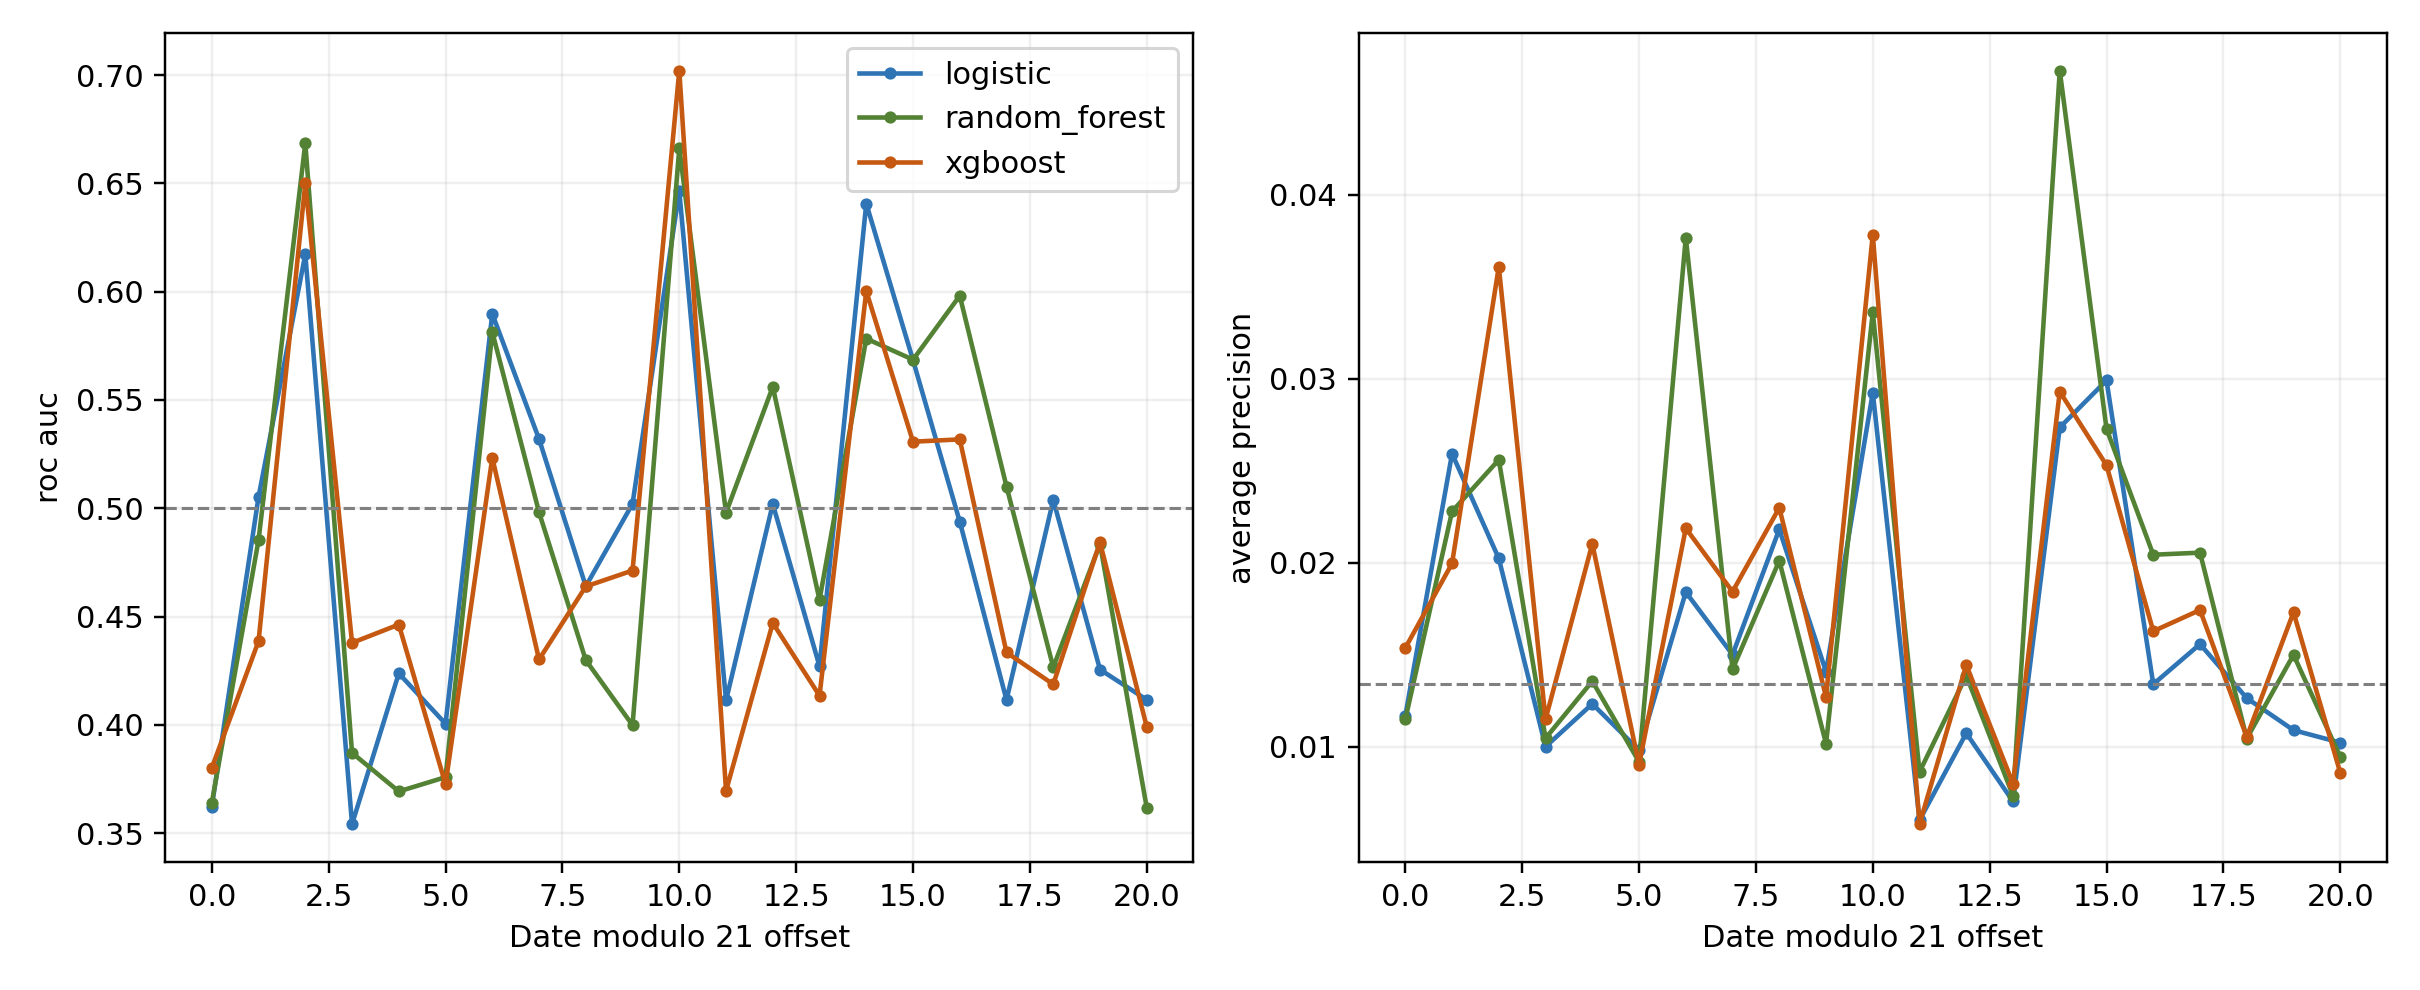
\includegraphics[width=0.88\textwidth]{nonoverlap_21offsets.png}
\caption{Performance across all 21 non overlapping Date-modulo-21 offsets, averaged over three athlete-group allocations}
\label{fig:nonoverlap}
\end{figure}

\begin{multicols}{2}

In the prohibited-feature leakage stress test, recording gap alone achieved mean ROC-AUC 0.983 and AP 0.519; adding the safe predictors yielded ROC-AUC 0.985 and AP 0.527. In contrast, the safe primary logistic control achieved approximately ROC-AUC 0.614 and AP 0.018. The administrative observation pattern was therefore far more predictive of the supplied label than the intended training-load predictors.

The observed safe logistic refit achieved ROC-AUC 0.6207 and AP 0.0187. Under 100 within-athlete random permutations, the null means were 0.5418 and 0.0156, with empirical $p=0.0099$ for both metrics. Under 100 within-athlete circular shifts, null means were 0.5335 and 0.0152, with empirical $p=0.0099$ and $p=0.0198$. The full-window data thus contained structured association beyond these label controls, but that association did not survive temporal de-overlap.

Adding the three raw relative-load ratios to an otherwise identical logistic sensitivity model changed mean ROC-AUC from 0.612 to 0.624 and AP from 0.019 to 0.021. This small exploratory difference was not used to redefine the primary feature contract.

Across fixed budgets of 1-10 alerts per 100 rows, observed precision ranged from 0.23\% to 1.89\%. Athlete-bootstrap intervals overlapped the 1.34\% prevalence baseline. At 10 alerts per 100, recall was 12.0\% for logistic regression, 14.1\% for random forest, and 12.2\% for XGBoost, while precision remained 1.61\%, 1.89\%, and 1.64\%. No evaluated policy supported automated training restriction or clinical escalation.

Across the 15 repeated outer fits, mean pairwise feature-rank Spearman correlation was 0.480 for logistic regression, 0.886 for random forest, and 0.428 for XGBoost; mean top-10 Jaccard overlap was 0.389, 0.634, and 0.395. Random-forest reliance rankings were more stable, but stable rankings cannot be interpreted as physiological or causal explanations when non-overlapping predictive performance is at chance.

%===========================================================================
\section{Discussion}
%===========================================================================

This reanalysis changes the scientific interpretation without disputing that the published weekly discrimination can be reproduced. The source-style protocol yielded ROC-AUC 0.677, closely matching the originally reported 0.678 \cite{lovdal2021}. The methodological question is therefore not whether the published score can be reconstructed, but whether that score estimates the claimed generalization setting. Three progressively stronger checks address this question: removal of test-cohort distribution information and separation of model-development operations from evaluation; athlete-disjoint nested validation with calibration assessed independently of fitting; and explicit evaluation of all 21 non-overlapping temporal offsets. Together, these tests show that the headline discrimination is not robust to validation designs intended to represent unseen-athlete use.

The principal methodological contribution is therefore the validation-integrity audit rather than a new injury-prediction model. Existing guidance and prior studies have identified individual risks such as data leakage, inadequate participant separation, temporal dependence, and calibration problems \cite{vaneetvelde2021,kapoor2023,collins2024,moons2025}. Our audit differs by treating these concerns as executable stress conditions within one longitudinal protocol and by testing whether correcting each condition changes the inferential claim. The controlled null simulations establish that participant memorization and global supervised selection can create apparent discrimination when no population-generalizable signal exists. The independent cohort then shows that the same classes of validation sensitivity recur across linear, bagged-tree, and boosted-tree models. The result is a methodological finding about the integrity of validation claims, not a claim that any single model family is intrinsically unreliable.

The controlled null simulations establish mechanism under known ground truth: participant memorization and whole-dataset selection generated apparently useful discrimination when no signal could generalize. The independent cohort then reproduced validation sensitivity across linear, bagged-tree, and boosted-tree models. Random row validation allowed nearly every participant identity to occur on both sides of each split and materially inflated performance, especially for flexible tree ensembles. Whole-dataset supervised selection introduced additional optimism even after participant grouping. Together, the simulation and two cohorts convert a dataset-specific reanalysis into a methodological result.

The recording-gap leakage stress test provides the clearest evidence that the observation process matters. An administrative feature achieved AP 0.519 compared with approximately 0.018 for the safe predictors. Together with the exact 22-unit spacing before most positive-run starts, this suggests that missing or retained rows encode how the event-centred table was constructed. Such variables can act as proxies for events or post-event data availability, creating impressive but scientifically invalid performance.

The results are consistent with broad concerns about data leakage and overoptimistic validation in ML-based science \cite{kapoor2023}, as well as sports-injury reviews that call for stronger temporal and external validation \cite{vaneetvelde2021,leckey2025}. They also complement, rather than duplicate, the recent daily-file study by Qiao and Tian \cite{qiao2026}. That work evaluated seven-day sequences and temporal deep learning; the present study directly reproduces the published weekly protocol, identifies its test-outcome-dependent normalization, quantifies the exact 21-day observation structure, evaluates all 21 weekly offsets, and then tests identity and feature-selection leakage in an independently collected cohort. More broadly, recent trustworthy-AI audit work has shown the value of explicitly testing leakage mechanisms in medical prediction, but has focused on rule-derived label leakage and a different application domain \cite{benammar2026}. The present audit is narrower in scope and specifically targets the validation threats created by repeated identities, longitudinal histories, outcome-informed operations, calibration, and observation processes.

Wu and colleagues transparently noted that feature ranking on their complete dataset could introduce leakage \cite{wu2026}. Our audit quantifies that concern and identifies participant mixing as a second, often larger source of optimism. This does not invalidate the value of their prospective multidisciplinary data; it shows why the unit of generalization and locality of supervised operations must match the claimed use setting. Algorithm complexity alone is not the decisive factor.

Four practices emerge. First, the prediction time and target risk set must be defined before feature engineering. Second, every preprocessing statistic must be estimated without test outcomes, and repeated measurements from the same athlete must remain grouped. Third, adjacent windows should be explicitly audited; when histories overlap, a non-overlapping evaluation should accompany the full-window result. Fourth, discrimination should be reported with calibration, prevalence-relative skill, uncertainty, and alert burden. These practices operationalize the transparency principles of TRIPOD+AI and the risk-of-bias concerns of PROBAST+AI \cite{collins2024,moons2025}.

We recommend reporting these properties as a validation-integrity profile rather than collapsing them into a single score: identity separation, transformation locality, supervised-selection locality, calibration independence and prevalence alignment, temporal-history independence, and observation-proxy resistance. A composite score could conceal one fatal violation; the profile makes each claim auditable and supplies executable stress tests.

Negative results under these safeguards are scientifically valuable. They prevent a retrospective association from being marketed as prospective prevention, expose limits of the available data, and indicate which new data collection would be informative. In this case, the next model-development step is not a larger neural network. It is a continuously observed prospective cohort with documented injury onset, recovery, recurrence, time-varying availability, and an external validation site.

Strengths include exact source-file verification, reproduction before correction, a prespecified feature contract, repeated nested athlete-level validation, independent calibration, cluster-aware uncertainty, all 21 non-overlapping offsets, two refitted label controls, a deliberate observation-process stress test, complete out-of-fold prediction retention, and replication of validation sensitivity in a second prospective cohort and three model families. The study evaluates not only whether models rank cases, but whether their probabilities and alerts are useful.

Several limitations remain. In cohort 1, the endpoint is supplied rather than clinically reconstructed and may contain repeated rows from the same injury episode. The event-centred sampling mechanism cannot be fully recovered, so causal statements about why rows are missing are not possible. Only 74 athletes were available, and the final-10 comparison had 10 independent clusters. In cohort 2, participant identifiers were reconstructed from invariant baseline fingerprints because the processed release omitted both ID and week; exact agreement across both matrices and contiguous runs supports the reconstruction, but does not replace a documented identifier. The missing week field prevented prospective temporal validation. Our fixed-model external audit is not an exact reproduction of the publication's extensive tuning workflow, and the second cohort validates the audit mechanism rather than transport of one common model. Calibration and bootstrap intervals quantify within-cohort uncertainty, not clinical transportability. Finally, feature-importance stability measures model reliance, not causal injury determinants.

\end{multicols} 

%===========================================================================
\section{Conclusion}
%===========================================================================

Across two runner cohorts, apparently moderate sports-injury AI performance was not robust to validation designs matching unseen-athlete use. In the first cohort, test-distribution access, prevalence-mismatched calibration, temporal overlap, and recording structure changed the conclusion. In the second, participant mixing and global supervised selection inflated performance across model families. The evidence supports an executable trustworthy-AI validation framework, not a deployment-ready injury-warning system. Future work should use explicit participant and time identifiers, prospective risk sets, external-site transport validation, and decision-linked evaluation before further algorithmic optimization.



\newpage 
%===========================================================================
\section*{Statements and Declarations}
%===========================================================================

\subsection*{Ethics approval:} This study is a secondary analysis of publicly released, de-identified data and required no new participant contact. The original cohort-1 creators report approval under research code PSY-1920-S-0007 \cite{lovdaldataverse2021}; ethics and consent procedures for cohort 2 are reported by Wu and colleagues \cite{wu2026}.

\subsection*{Consent for publication} Not applicable.

\subsection*{Data availability:} The first cohort and official replication notebook are available from DataverseNL under DOI \href{https://doi.org/10.34894/UWU9PV}{10.34894/UWU9PV} \cite{lovdaldataverse2021}. The processed matrices for the second cohort are official supplementary files to DOI \href{https://doi.org/10.1038/s41746-026-02413-y}{10.1038/s41746-026-02413-y} \cite{wu2026}. Source hashes and provenance are included in the reproducibility package; redistribution terms must be confirmed before public archiving.

\subsection*{Code availability:} All code required to reproduce the analyses, simulations, validation protocols, figures, and summary tables is available at \href{https://github.com/aboutara-marouane/validation-integrity-sports-injury-ai}{https://github.com/aboutara-marouane/validation-integrity-sports-injury-ai}. The repository includes pinned software dependencies, master random seeds, source-data hashes, feature manifests, split assignments, and instructions for obtaining the original data from their respective repositories. Source datasets are not redistributed; their access and reuse are governed by the terms of the original data providers.

\subsection*{Funding:} The authors received no specific funding for this study.

\subsection*{Competing interests:} The authors declare no competing interests.

\subsection*{Author contributions:} M.A.-B.: conceptualization, methodology, software, validation, formal analysis, visualization, writing original draft. M.Z.E.-s. and S.B.: supervision, methodological review, and writing review.


\newpage
\bibliographystyle{unsrt}
\bibliography{references}

\end{document}
